\section{Kernel construct for convolutions}
\label{sec:kernelconstruct}

\subsection{Surface code kernels and symmetry considerations}
\label{sec:kernels}


With ideal weight initialization and activation functions across its layers, a multilayer perceptron from the $(d^2-1)\times r$ inputs of a QEC cycle should always provide the optimal predictions for the probabilities of the error states of logical observables. The size of such a network grows at best linearly with both $d^2$ and $r$, so larger-distance surface codes, or QEC cycles with more rounds, become infeasible to implement in hardware acceleration devices. The purpose of defining kernels for a convolutional NN structure is to keep the growth of the number of NN parameter in spatial dimensions fixed by sharing weights explicitly as the kernels are evaluated across their stride through the full surface code. The approach described in this paper uses smaller surface codes of distance $k$ as kernels and defines a rule to combine their output; in this way, the growth of the NN along spatial dimensions is fixed at $\Order(k^n)$ in spatial dimensions, with a fixed integer $n=4$ or 6 depending on the representation of the relationship between the inputs and the outputs of the kernel, see more discussion on this point in Section~\ref{sec:kernels-r2}.
Odd-$k$ kernels are the only ones that can provide total coverage for both odd- and even-$d \geq k$ surface codes, and $k=3$ keeps the number of NN parameters minimal while providing sufficient error decoder performance.

In typical image recognition applications, pixels are arranged in a regular grid, and edge effects on smearing are usually ignored. In our case, however, noise mechanisms are more complex, with single-qubit operations affecting data and measure qubits independently, and two-qubit operations causing correlated errors between data and measure qubits. For this reason, we cannot ignore edge effects (or lack thereof). 
In a surface code with no holes, accounting for edges necessitates the use of 5 different kernels. As illustrated on the left panel of Fig.~\ref{fig:ktypes}, we classify these kernels as \type{0} when facing both top and left edges of the surface code, \type{1} when facing only the top edge of the surface code, \type{2} when facing both top and right edges of the surface code, \type{3} when facing only the left edges of the surface code, and \type{4} when being fully immersed in the surface code with full connectivity to other data and measure qubits at the kernel boundaries. We note that strides of kernel evaluations along the bottom or right edges (bottom right and bottom left corners) of the surface code are equivalent to evaluating \type{1} and \type{3} (\type{0} and \type{2}) kernels with the order of inputs and outputs rotated by $180\degrees$, and that moving the same kernel type one step in measure and data qubits up/down or left/right for the evaluation of the next stride in these directions requires mirroring the order of inputs and outputs along either the vertical or horizontal direction -- we choose the former in our implementation. We further note that even-$d$ surface codes cannot have \type{2} kernels as the arrangement of measure qubits in these surface codes is such that the top right corner is identical in edge conditions to the flipped configuration of the \type{0} kernel. The simplest such even-$d$ surface code that can be evaluated through $k=3$ kernels is a $d=4$ surface code, and the different strides over the only \type{0} kernel needed for this surface code is illustrated on the right panel of Fig.~\ref{fig:ktypes}.

%%%%%%%%%%%%%%%%%%%%%%%%%%%%%
\begin{figure*}[htb]
\centering
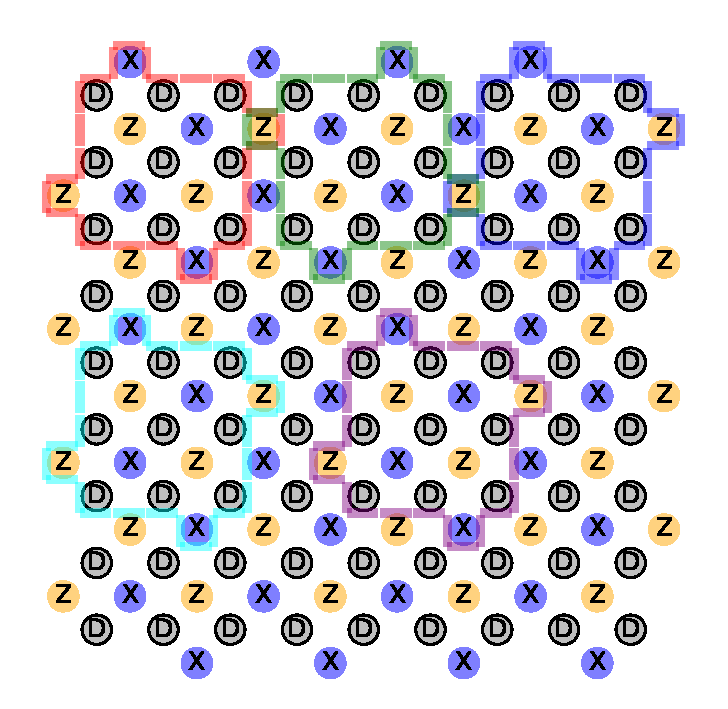
\includegraphics[width=0.45\textwidth]{kernel_types.pdf}
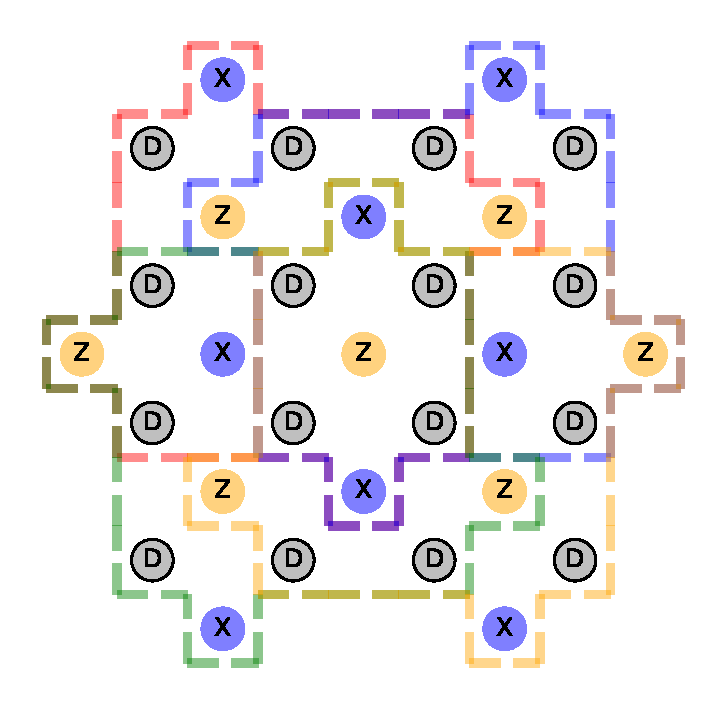
\includegraphics[width=0.45\textwidth]{d4_kernels.pdf}
\ccaption
{Kernel types}
{
Illustrated over a $d=9$ surface code on the left are the five types of kernels used in this paper, displayed using boundaries with different colors (type-0: red, type-1: green, type-2: blue, type-3: cyan, and type-4: purple). The types are based on whether the kernel edges face a boundary of the full surface code or other data qubits. The green kernel is shown in flipped configuration while the others are in standard arrangement.
The overlap of single-step kernel strides are illustrated on the right over a $d=4$ surface code. In this case, the type of the kernels used in each stride is the same (type-0, \ie, red kernel on the left panel), and the boundaries with different colors only highlight the strides. The strides are constructed using standard (red and gold strides) or flipped (blue and green) configurations with either a 180\degrees{}-rotation (gold, green) or none (red, blue).
In both panels, the data and measure qubits are shown with color-coded circles and are marked with letters `D' (data qubits, gray), `X' (measure-$X$ qubits, blue), or `Z' (measure-$Z$ qubits, gold).
}
\label{fig:ktypes}
\end{figure*}
%%%%%%%%%%%%%%%%%%%%%%%%%%%%%

While error probabilities at each data or measure qubit may not be distributed uniformly in hardware, we assume uniformity across the symmetry axes of the kernels or the evaluations of the same kernel type at different strides in order to encode the fundamental spatial symmetries of the surface code and reduce the number of free parameters of the model. As kernels provide basic relationships between the stabilizer measurements over the measure qubits and the error states of the data qubits at a fundamental level, regardless of how the input over the measure qubit readings is represented or whether there are any hidden layers, symmetries within the kernel can, therefore, also be considered to reduce the number of parameters even further. 

In the cases we consider, \type{4} kernels are symmetric for a $180\degrees$-rotation, so the relations between measure and data qubits should also be established as such.
These relations are illustrated in Fig.~\ref{fig:t4kernslsym}, where one may conceptualize the displayed relationships $\mathcal{R}_{ij}$ in a simple way as NN weights that are shared between the data qubits according to the present rotational symmetry and are multiplied by a different ordered vector of measure qubit readouts to produce the same kernel output dimensionality as the other kernel types. 
Note that Fig.~\ref{fig:t4kernslsym} does not represent a concrete transformation in the NN --- rather, it is meant to illustrate \emph{how} one might formalize the symmetric nature of the weights.
As will be discussed in Section~\ref{sec:kernels-r2}, our architecture implements a quadratic polynomial over the stabilizer measurements, and the symmetry relationships are analogous to this concept.


%%%%%%%%%%%%%%%%%%%%%%%%%%%%%
\begin{figure*}[htb]
\centering
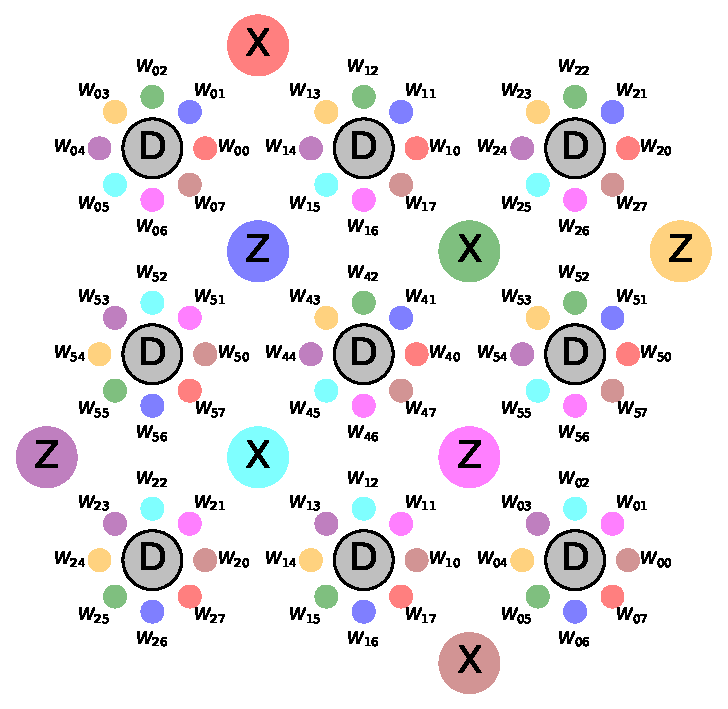
\includegraphics[width=0.6\textwidth]{symmetric_kernel_output_relation.pdf}
\ccaption
{Symmetries in the input--output relations of the type-4 kernel}
{
The relations are illustrated in a $k=3$ kernel. Each measure qubit is represented with a circle that is filled with a different color while the data qubits are represented with gray-filled circles. The weights used in evaluating the relationship of each data qubit to the measure qubits is denoted in an abstract way through the symbols $\mathcal{R}_{ij}$, where index $i$ is the index of the output, and index $j$ is the index of the position of the ordered input passed. One should note that the allowed values of $i$ only go up to 5 because of the symmetrization of weights even though there are 9 data qubits in the kernel, with relations only for $i=4$ being unique. The small filled circles around the data qubits color-code how the input order in these relationships match the physical measure qubit positions.
}
\label{fig:t4kernslsym}
\end{figure*}
%%%%%%%%%%%%%%%%%%%%%%%%%%%%%

\subsection{Input representations over multiple rounds}
\subsubsection{Input representation over two or less rounds}
\label{sec:kernels-r2}

In assessing whether an error occurred in data qubits or measure qubits, it is important to examine stabilizer measurements and their changes over successive rounds, and correlate these changes spatially.
Since stabilizer measurements and detector events are a series of 0s and 1s, one can encode pairwise correlations across spatial and temporal directions into matrices using a quadratic representation over the inputs.

For $k=3$, we find a quadratic representation sufficient to encode the correlations over $r \leq 2$ rounds --- by which we mean spatially, or, independent of the evolution of time (passage of rounds).
The quadratic representations of the stabilizer measurements and detector events are kept disjoint in the architecture via different embedding layers, and each kernel type constructs its own independent embedders, \ie, each kernel type maintains an independent set of trainable embedding weights:
\begin{itemize}
\item Stabilizer measurement embedding: For distinct measure bits $m_i$ and $m_j$, the quadratic representation is computed as
\begin{equation}
\begin{aligned}
b_{ij}&=(m_i+1) \cdot (m_j+1) - 2 \\
q_{ij}&=(p_{ij}+1)/2 \\
r_{ij}&=-q_{ij} \cdot b^2_{ij} + q_{ij} \cdot b_{ij}+ p_{ij},
\end{aligned}
\end{equation}
where $p_{ij}$ are $p$-like NN parameters, and $r_{ij}$ is the result of the quadratic correlation of the bits at positions $i$ and $j$. 
In this way, when both $m_i$ and $m_j$ are 0 or 1, $r_{ij}=-1$, and when they are different, $r_{ij}=p_{ij}$.
Because the actual values of stabilizer measurements are not informative, we do not include quadratic representations for the $i=j$ diagonal terms.
\item Detector event embedding: For arbitrary, distinct detector event bits $e_i$ and $e_j$ (we will discuss the specifics of the events later), the quadratic representation is computed as
\begin{equation}
\begin{aligned}
b_{ij}&=(e_i+1) \cdot (e_j+1) - 2 \\
q^{(0)}_{ij}&=\left(p_{ij}\cdot\left(x_{ij}+1 \right)-1\right)/2 \\
q^{(+)}_{ij}&=x_{ij}/6 \\
r_{ij}&=(-q^{(0)}_{ij}+q^{(+)}_{ij}-1/3) \cdot b^2_{ij} + (q^{(0)}_{ij}+q^{(+)}_{ij}+2/3) \cdot b_{ij}+ 2 \cdot q^{(0)}_{ij},
\end{aligned}
\end{equation}
where $p_{ij}$ and $x_{ij}$ are $p$-like and $x$-like NN parameters, respectively, and $r_{ij}$ is again the result of the quadratic correlation of the bits at positions $i$ and $j$.
Using this representation, $r_{ij}=-1$ if $e_i=e_j=0$, $r_{ij}=x_{ij}$ if $e_i=e_j=1$, and $r_{ij}=p_{ij}\cdot\left(x_{ij}+1 \right)-1$ otherwise, thereby bounding the values flexibly between -1 and $x_{ij}$.
When the quadratic representation of the stabilizer measurements include correlation terms across consecutive rounds, we do not include the diagonal terms for $i=j$; when this is not the case, the bits are simply mapped as $0\to -1$ and $1\to1$ for these diagonal terms.
\end{itemize}

In the actual computations, because these matrices are symmetric, we take only the upper-triangular elements (excluding the diagonals) and flatten them for use with fully-connected networks.

We should note that considerations for symmetry in \type{4} kernels, discussed in Section~\ref{sec:kernels}, also apply to embedding layers. In this case, however, the embedding weights are those that need to respect a $180\degrees$-rotation. Our architecture accounts for this symmetry consideration as well to maximize the sharing of NN weights.

After the kernel input is passed through the embedding layers, the kernel output is determined through a single, dense layer of weights over the output of these embedders. Referring to the kernel types mentioned in Section~\ref{sec:kernels}, kernels of \texttt{types} 0--3 have $k^2$ outputs whereas \type{4} kernels have $(k^2+1)/2$ outputs, remapped to $k^2$ outputs based on symmetry considerations.


\subsubsection{Input representation over three rounds or more}
\label{sec:kernels-r3}

Under noiseless conditions, measure qubits are expected to remain in the same state at each error correction cycle.
In the series of measurements of a measure qubit, a single bit flip such as that in a measurement sequence $0001000$ of $r=7$ cycles would result more likely from an error in the measure qubit than two consecutive errors in a data qubit, which would also be correlated with the sequence of another measure qubit.
A sequence of $0001011$, on the other hand, is more likely to indicate a data qubit error, followed by an error in the measure qubit, than three errors in the measure qubit itself.
These cases can be represented easily with \type{C} detector events, the sequence of which, in these two examples, would be $001100$ and $001110$, respectively. An odd parity in such a sequence would potentially signal data qubit errors.

There are, however, cases where an odd parity in detector events might be ambiguous to interpret on their own. Take for example the sequence $1000000$ of measure qubit states. In this case, an error could have occurred in an adjacent data qubit between rounds 1 and 2, or the first measurement of the measure qubit might have been erroneous. In both cases, correlations with the states of other measure qubits would need to be checked, and with additional errors in these states, frame shifts in where correlated errors occur could be possible.

When there are three or more rounds of measurements, one can access a representation of the evolution of states that can be interpreted probabilistically; this representation can be used in a recurrent architecture that takes triplets of stabilizer measurements (doublets of detector events) as input in layers that ensure recurrent behavior. 
In order to do so, we need to define a stabilizer triplet state and an algorithm for the evolution of this state based on a moving window of triplets of measure qubit states --- see Algorithm~\ref{alg:state_evolution} for the subroutine used to produce the states. Note this algorithm also computes a set of change values that are used for internal book-keeping and then discarded.

\begin{algorithm}
\caption{Triplet state evolution}
\begin{algorithmic}[1]
\For{triplets of rounds with a time stride of one round}
  \For{each measure qubit}
    \If{this is the first triplet}
      \State initialize the triplet state as $s=-1$ and a change vector $v=1$.
    \EndIf
    \If{the triplet contains identical measurements}
      \State $s$ and $v$ do not change.
    \Else
      \If{the first and third measurements are the same} 
        \State $v$ changes sign, but $s$ remains the same.
      \Else
        \State update the state as $s+v$ and bound between $-1$ and $1$.
      \EndIf
    \EndIf
    \If{the state $s$ reaches the boundaries $\pm1$}
      \State $v$ is reset to $-s$.
    \EndIf
  \EndFor
\EndFor
\end{algorithmic}
\label{alg:state_evolution}
\end{algorithm}

For illustration, here are a few examples of triplet state evolutions from measure qubit sequences for arbitrary individual measure qubits:
\begin{itemize}
\item Measurements: $000010000$; states: $-1,-1,0,0,-1,-1,-1$.
\item Measurements: $000011000$; states: $-1,-1,0,1,0,-1,-1$.
\item Measurements: $000010111$; states: $-1,-1,0,0,0,1,1$.
\item Measurements: $000001111$; states: $-1,-1,-1,0,1,1,1$.
\item Measurements: $000011111$; states: $-1,-1,0,1,1,1,1$.
\item Measurements: $000011011$; states: $-1,-1,0,1,0,1,1$.
\item Measurements: $100000000$; states: $0,0,0,0,0,0,0$.
\item Measurements: $000000001$; states: $-1,-1,-1,-1,-1,-1,0$.
\item Measurements: $100000001$; states: $0,0,0,0,0,0,1$.
\item Measurements: $100010001$; states: $0,0,1,1,0,0,-1$.
\item Measurements: $100011001$; states: $0,0,1,0,-1,0,1$.
\end{itemize}
An example set of such triplet states and accompanying detector events are also displayed in Fig.\ref{fig:d5r5states} for a $d=5$ code with $r=5$ rounds.

%%%%%%%%%%%%%%%%%%%%%%%%%%%%%
\begin{figure*}[htb]
\centering
~~~~~~~~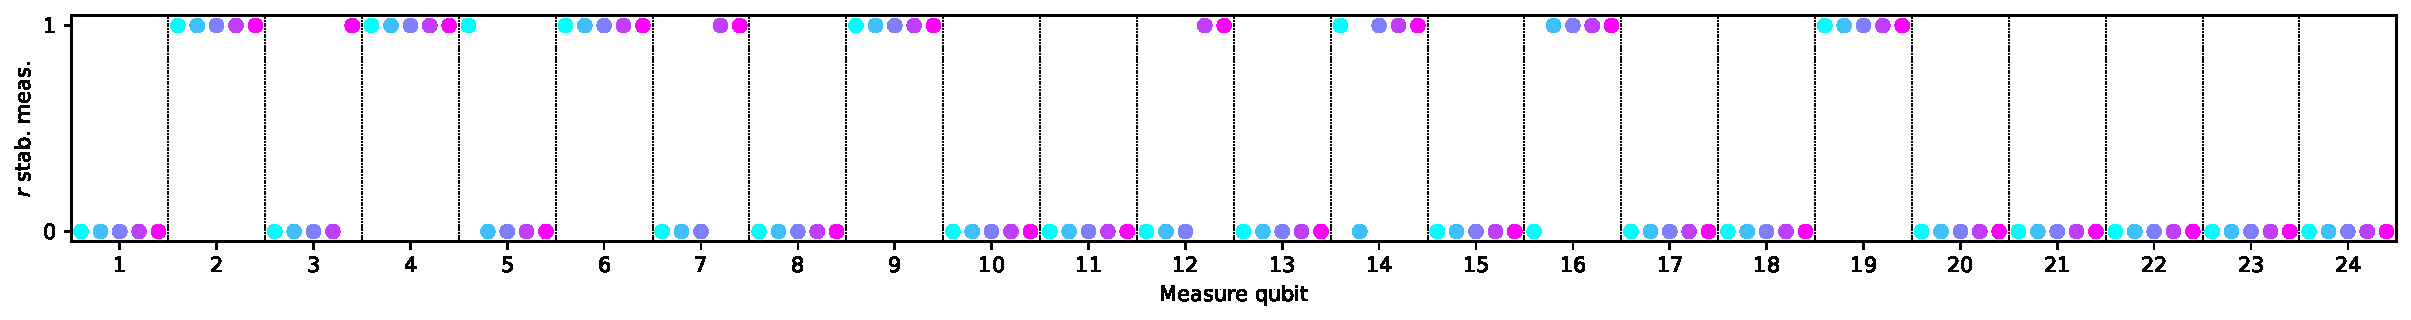
\includegraphics[width=0.9\textwidth,left]{stabilizers_d5_r5_event0.pdf} \\
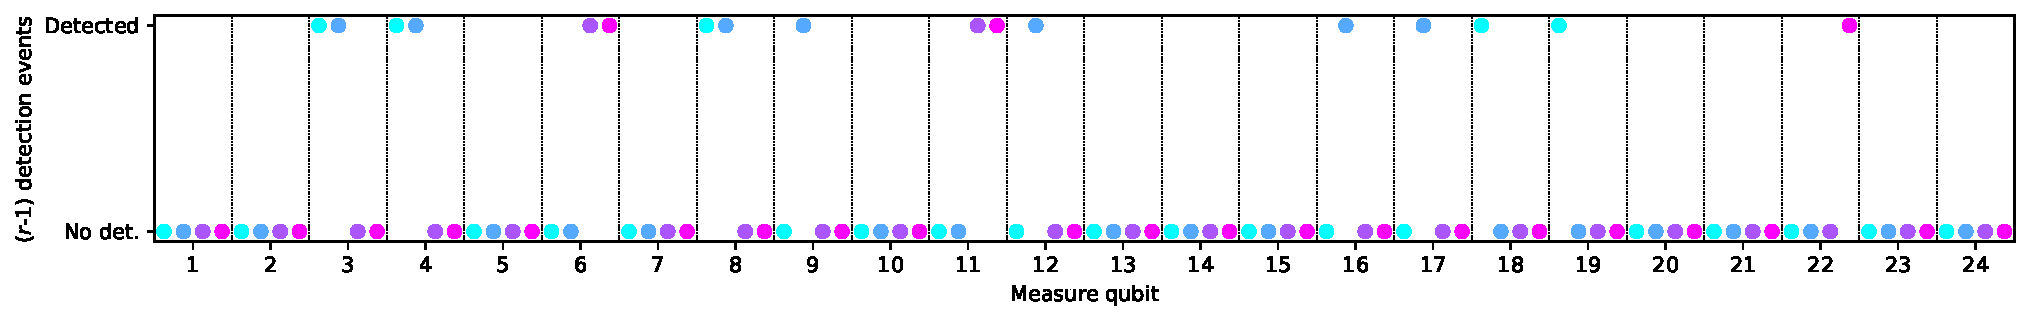
\includegraphics[width=0.7573\textwidth,left]{det_evts_d5_r5_event0.pdf} \\
~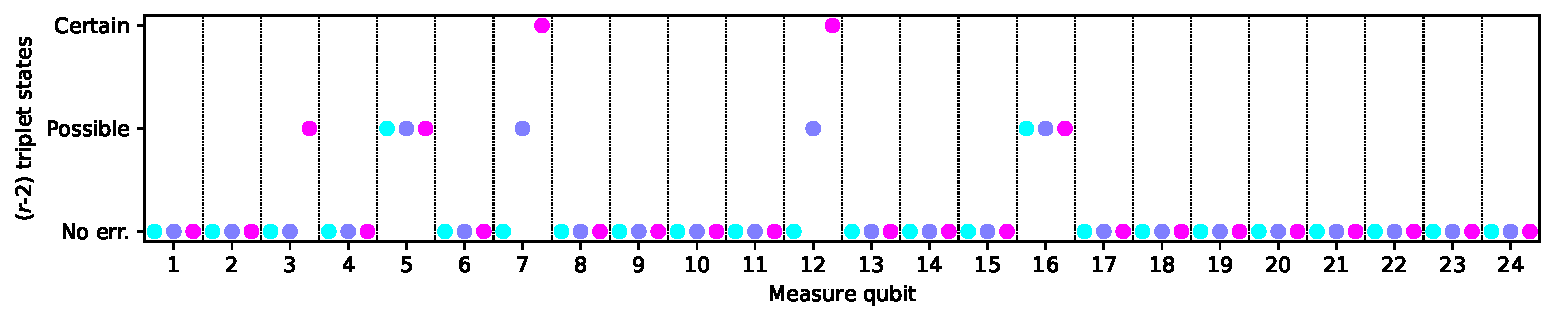
\includegraphics[width=0.5804\textwidth,left]{states_d5_r5_event0.pdf}
\ccaption
{Comparison of stabilizer measurements, detector events, and triplet states}
{
Displayed are the stabilizer measurements (top), detector events (middle), and triplet states (bottom) from $r=5$ rounds of stabilizer measurements over the 24 measure qubits of a $d=5$ code. The horizontal axis in all panels is divided by dotted lines for each measure qubit, and the successive stabilizer measurements (5 measurements), detector events (4 \type{C} events), and (3) triplet states are coded with different colors. The detector events are interpreted as having no detection ($e=0$) or having detected an error ($e=1$), and the triplet states are interpreted as no error ($s=-1$), possible error ($s=0$), and certain error ($s=1$).
}
\label{fig:d5r5states}
\end{figure*}
%%%%%%%%%%%%%%%%%%%%%%%%%%%%%

When converting the ensemble of states at each round into an embedded input vector of probabilities, we consider pairs of $(s_i, s_j)$ with all $j\leq i$ (of which there are $m^2\left(m^2-1\right)/2$ pairs for a distance-$m$ code). 
This quadratic embedding representation replaces the stabilizer measurement embedder discussed in Section~\ref{sec:kernels-r3} while keeping the detector event embedder and the succeeding dense layer, which produces the final kernel output, the same.
We define a function $f_s$ such that when $i=j$, \ie, $f_s(s_i, s_i)$:
\begin{equation}
\begin{aligned}
f_s(1,1) &= 1 \\
f_s(0,0) &= p_i \\
f_s(-1,-1) &= -1
\end{aligned}
\end{equation}
When $i \neq j$, we have:
\begin{equation}
\begin{aligned}
f_s(1,1) &= 1 \\
f_s(1,0) &= p_{ij,0} \\
f_s(0,-1) &= p_{ij,0} \times p_{ij,1} \\
f_s(1,-1) &= p_{ij,0} \times \left(p_{ij,2} + p_{ij,1} \times \left(1-p_{ij,2}\right)\right) \\
f_s(0,0) &= p_{ij,0} \times \left(p_{ij,3} + p_{ij,1} \times \left(1-p_{ij,3}\right)\right) \\
f_s(-1,-1) &= 0
\end{aligned}
\end{equation}
Here, the parameters $p_i$ and $p_{ij,\mu}$ are trainable $p$-like NN parameters. In order to avoid the scaling of the number of parameters by a leading factor of $d^4$, we construct this embedding for each kernel separately, \ie, $m=k$, which is a fixed number, instead of $m=d$, which could be significantly larger than $k$. As in other embedding layers, these parameters are also required to respect the rotational symmetry of the type-4 kernels.

The probabilistic output $\vec{p}$ of this triplet state embedder is converted to $2\vec{p}-1$ and combined with the output of the detector event embedder before passing through the dense layer of a kernel for final kernel output processing. We will see further in Section~\ref{sec:rcnn} how the triplet state embedder is placed within the recurrent NN structure.
